\section{More on TLS}

\subsection{TLS Overview}

\paragraph{High Level Goals}
TLS aims for security in face of an attacker with complete control of the network. The only requirement for the underlying transport is a reliable and in-order data stream (TLS is between the transport and application layer).
\begin{itemize}
    \item \textbf{Entity Authentication:} Server side is always authenticated, client side optional. Authentication via asymmetric crypto (signatures) or symmetric pre-shared key (unique for each session).
    \item \textbf{Confidentiality:} Data only visible to the endpoints, but TLS does not hide length of data (padding possible).
    \item \textbf{Integrity / Reliability:} Data cannot be modified without detection. Guarantees also cover reordering, insertion and deletion.
\end{itemize}

\paragraph{Part 1: Handshake Protocol}
Used by client and server to negotiate cipher suite\footnote{Click \href{https://ciphersuite.info/cs/}{link} for a list of all 337 cipher suites and their security status.} (set of algorithms to secure the connection, e.g. key exchange, encryption, MAC, etc.), authenticate each other (certificates and public keys) and establish session keys used in the Record Protocol (see below).

\paragraph{Establishing Session Keys}
The client either encrypts a random number with the server's public key, with which both parties generate a unique key or the client uses a Diffie-Hellman key exchange (see previous Section). The second option has the property of forward secrecy.

\paragraph{Forward Secrecy}
Future disclosures of encryption keys cannot be used to decrypt communications recorded in the past. More specifically. session keys cannot be compromised even if long-term secrets used in the session key exchange are compromised. Additionally, compromising unique session keys should not affect any other communications encrypted with a different session key. Assumes passive attacks, i.e. does not protect against an active MITM attack.

E.g.: In HTTPS, the long-term secret is typically the private signing key of the server.

\paragraph{Part 2: Record Protocol}
Using the session keys established in part 1, the application layer communication is guaranteed to be confidential and reliable. 

The Record Protocol provides a stream-oriented API (fragmentation/coalescence of data allowed). A record is a TLS data unit, which is a fragment of the data stream.

\paragraph{Cryptographic Protections in the Record Protocol}
\begin{itemize}
    \item Data origin authentication.
    \item Data integrity using a MAC.
    \item Data confidentiality using a symmetric encryption algorithm (integrity and encryption combined in TLS 1.3 by use of AEAD).
    \item Prevention of reflection attacks by key separation (different symmetric keys in different directions).
\end{itemize}

\paragraph{Reflection Attack}
Attacking a challenge-response authentication system that uses the same protocol in both directions by tricking the target into providing the answer to its own challenge.

\paragraph{TLS 1.0 (1999)}
First version of TLS (after migrating from SSL) and deprecated in 2020 due to security flaws.

\paragraph{TLS 1.1 (2006)}
Fixed the security flaws of version 1.1, such as protection against cipher-block chaining attacks.

\paragraph{TLS 1.2 (2008)}
Changed hash algorithms used for the protocol, enhanced cipher suite negotiation abilities between client and server, support for authenticated encryption ciphers (see AE(AD)), addition of AES cipher suites, etc.
In 2011, backward compatibility with SSL was removed to prevent version fallback.

\begin{figure}[h]
	\centering
	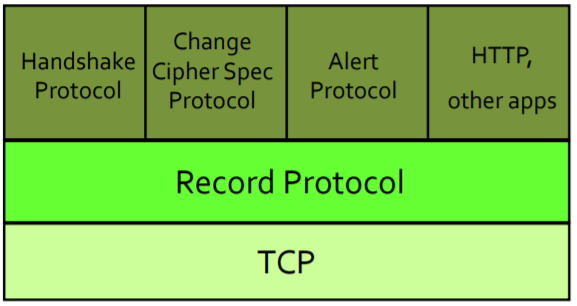
\includegraphics[scale=0.4]{images/3-tls12.PNG}
	\caption{TLS 1.2 protocol architecture.}
	\label{fig:tls12}
\end{figure}

\paragraph{TLS 1.2 Handshake}
When using TCP, the full handshake is a 3-RTT protocol (see Figure \ref{fig:poorhandshake}). 

\begin{figure}[h]
	\centering
	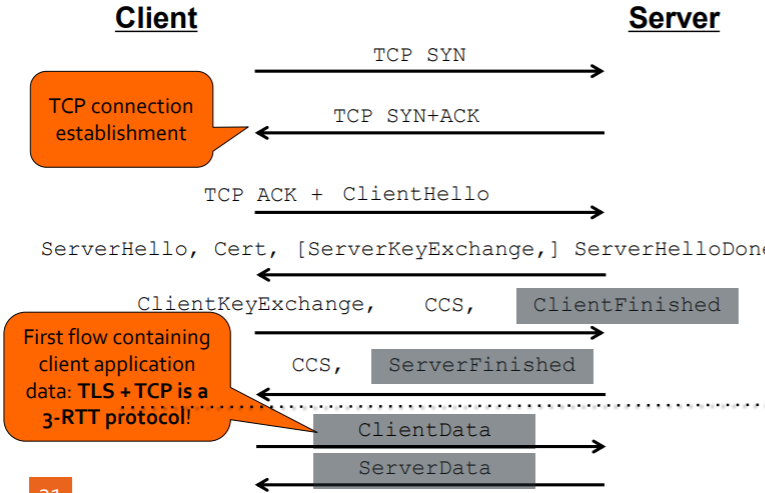
\includegraphics[scale=0.5]{images/3-poorhandshake.PNG}
	\caption{The full TCP + TLS 1.2 handshake.}
	\label{fig:poorhandshake}
\end{figure}

\paragraph{TLS 1.3 (2018)}
Not yet widely used. Significant change to the way of coordinating the cipher suites between machines (part of the Handshake Protocol) by reducing the number of messages needed (cannot be used for version 1.2 and vice versa - the numbers of suites is reduced from 337 to 5). The key agreement and authentication algorithms are separated from the cipher suites. Mandates forward secrecy. Also removed support for less secure algorithms and introduced further security measures. Dropped support for insecure obsolete features such as compression (enabled \textit{CRIME} attack), renegotiation, non-AEAD ciphers (previous versions support MtE), etc. Encrypts all handshake messages after the \textit{ServerHello}.

TLS 1.3 basically wants to mimic QUIC by achieving the same RTT profile (excluding TCP overhead since it is unavoidable for TLS). QUIC offers a native 1-RTT handshake and a 0-RTT mode.

Compared to previous versions where the complete handshake is in the clear, version 1.3 encrypts almost all handshake messages with a separate key, providing security to both passive and active attacks on both ends.

\begin{figure}[h]
	\centering
	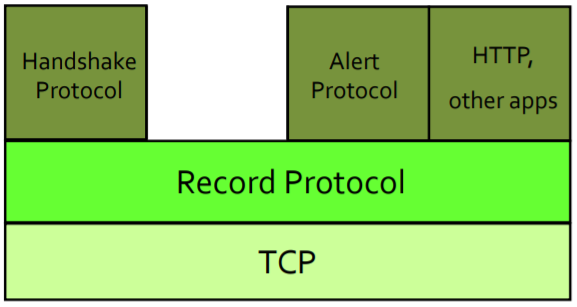
\includegraphics[scale=0.4]{images/3-tls13.PNG}
	\caption{TLS 1.3 protocol architecture.}
	\label{fig:tls13}
\end{figure}

\paragraph{Datagram TLS (TLS over UDP)}
Prevents eavesdropping, tampering or message forgery of UDP connection. Has to deal with fragmentation and packet reordering / loss. Avoids the \textit{TCP meltdown problem} when being used to create a VPN tunnel \footnote{\href{http://sites.inka.de/bigred/devel/tcp-tcp.html}{\textit{Why TCP over TCP Is A Bad Idea}}}.

\subsection{TLS 1.3 Details}

\paragraph{TLS 1.3 Record Protocol}
Each fragment is encoded into payload, ctype (single byte representing content type, i.e. handshake message, alert message or application data) and optional padding (used to hide true length of fragments). Encoded fragments are then encrypted using AEAD and appended to a record header.

For the AEAD encryption, a nonce is created by XORing the SQN and an IV. The 64-bit sequence number (SQN) is incremented for each record sent on a connection and maintained at each end of the connection (not included in header). The IV is a fixed per-TLS connection pseudorandom value derived from secrets established during the Handshake Protocol. XOR (masking) ensures that the nonce sequence is unique for each connection. This facilitates analysing security in a multi-connection setting.

The record header contains a 1-byte dummy type field, a 2-byte legacy version field (negotiated during handshake) and the length of the AEAD ciphertext (2 bytes).

AEAD-decryption failures are fatal and will lead to the connection being torn down and the key material being thrown away.

\paragraph{Attacks not Prevented by TLS 1.3 Record Protocol}
\begin{itemize}
    \item Truncation attacks on the stream of records.
    \item Application layer confusion.
    \item Timing attacks on the padding scheme.
\end{itemize}

\paragraph{TLS 1.3 Handshake Protocol}
Full handshake in 1 RTT (compared to 2 in 1.2 and earlier resp. 3 if TCP is counted. Achieved by only ever doing DH (elliptic or finite-field) and client speculatively sending several DH shares in supported groups (only a few) - server then picks one, replies with its share and Record Protocol keys can be derived. When resuming a previously established connection, a 0-RTT handshake is possible since shared state is kept with which a PSK can be derived. TLS 1.2 and earlier had the complete handshake in the clear, 1.3 encrypts almost all handshake messages and derives separate key to protect them (security for passive and active attacks).

%TODO DH shares, groups and curves? continuity

%TODO print out the slides for this part


\paragraph{Future of TLS}
%TODO: important? concluding remarks? largest security shifts


%TODO overview comparison to older versions? esp. handshake


